\section{Evaluation}
\label{sec:eval}

%%%%%%%%%%%%%%%%%%%%%%%%%%%%%%%%% 80 CHAR %%%%%%%%%%%%%%%%%%%%%%%%%%%%%%%%%%%%%%

\raj{break this up into lab based detailed power measurements and user study usability results. could be separate sections.}

%valuate the performance of {\myit} using a set of in-lab experiments 
%and an IRB-approved pilot study.

%%%%%%%%%%%%%%%%%%%%%%%%%%%%%%%%% 80 CHAR %%%%%%%%%%%%%%%%%%%%%%%%%%%%%%%%%%%%%%

\subsection{Controlled in-lab experiments}


The goal of our in-lab experiments is to show how each of {\myit}'s components 
contribute to the overall system performance.
%
To evaluate under realistic scenarios, we gathered 12 male and 5 female college
student volunteers to play the block stacking game (Section~\ref{sec:app})
with two modifications.
%
% First, instead of only using box-shaped blocks, our controlled in-lab experiments 
First, instead of using only box-shaped blocks, we
used cylinder-shaped blocks as well in addition to boxes.
%
While boxes are ideal for the purpose of measuring stereoscopsis levels, they 
are not suitable for validating the effectiveness of our mesh simplification
procedure, since a simplified box will still be a box.
%
Second, while the application for patients asks the users to stack five blocks,
we increase this number to 20 for non-patient users.
%
These changes to the application are made so that we have complex enough 
but controllable contents on the screen for fully utilizing and observing the 
benefits that {\myit}'s components offer.


While the volunteers participate,
we record the timestamp, head position, and head direction to formulate a 
``head tracking sample'' $HT_n$ for each participant.
%
Each $HT_n$ is used as a motion trace that we replay to further analyze the 
system-level performance, and in large, we categorized them into two levels of 
head motion; (1) small amount, and (2) large amount of head motions.
%
%\jk{DO WE NEED THIS? 
%Specifically, the position and direction information in $HT_n$ is translated
%to a translation matrix and rotation matrix, respectively.
%We pass the translation matrix through a linear interpolation and 
%the rotation matrix through a spherical linear interpolation to compute 
%the median value and re-position all the objects. 
%By doing so, we can replay the same display contents on the HoloLens 
%without physically moving the device.
%}
%
Using these traces, we analyze how different component and parameters in {\myit}
%such as binary tree-based mesh simplification, quad tree-based dynamics
%scoring, and culling, 
affects the energy usage performance of the HoloLens.


%%%%%%%%%%%%%%%%%%%%%%%%%%%%%%%%% 80 CHAR %%%%%%%%%%%%%%%%%%%%%%%%%%%%%%%%%%%%%%


\begin{figure}
    \centering
    \vspace{-1ex}
    \includegraphics[width=0.8\linewidth]{newMeshSimplificationEnergy}
    \vspace{-2ex}
    % \caption{Impact of binary tree depth $d_B$ on HoloLens energy 
    %         consumption with our block+cylinder stacking application, 
    %         compared with the case without {\myit}.}
    \caption{Impact of binary tree depth $d_B$ on energy 
            consumption compared with the case without {\myit}.}            
    \label{fig:meshsimplification-energy}
\end{figure}


%%%%%%%%%%%%%%%%%%%%%%%%%%%%%%%%% 80 CHAR %%%%%%%%%%%%%%%%%%%%%%%%%%%%%%%%%%%%%%

\spar{Binary Tree-based Mesh Simplification}:
%
We first measure the energy usage rate (mWh/10min) with and without {\myit}.
%
While doing this, we varied the binary tree depth $d_B$ of the mesh 
simplification algorithm to see how much complexity {\myit} can handle.
%
As \fig\ref{fig:meshsimplification-energy} confirms, {\myit} offers an energy
savings of up to $\sim$25\% compared to the case without {\myit}, reducing it
down close to the baseline usage rate ($\sim$490 mWh/10mins) of the 
platform even under minimal workloads.
%
This reduction holds even when a fairly deep binary tree ($d_B$=10) is 
constructed for 20 objects, which implies that our mesh simplification manages
to keep the computation (and energy) costs low.
%
Increasing depth $d_B$ does lead to a slight increase in energy usage since it
results in projecting more ``detailed'' objects, but insignificant up to a 
point where the computational load exceeds what can be handled by
the baseline limit. 
%
After this point, the energy consumption shows a steep increase. 
This is exemplified by a case where we doubled the number of objects on the 
scene (from 20 to 40) with $d_B$=10.

\begin{figure}[t]
    \centering
    \vspace{-2ex}
    \subfigure[Per second average frame rate when varying the frame dynamics 
                threshold for large amounts of motion.]{
        \includegraphics[width=0.8\linewidth]{newFrameDynamicsTraceLarge}
        \label{fig:framedynamics-trace-large}
    }
    \subfigure[Per second average frame rate when varying the frame dynamics 
                threshold for small amounts of motion.]{
        \includegraphics[width=0.8\linewidth]{newFrameDynamicsTraceSmall}
        \label{fig:framedynamics-trace-small}
    }
    \subfigure[Energy savings for varying dynamics thresholds.]{
        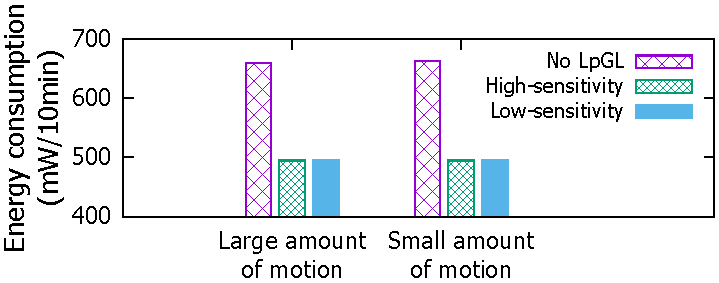
\includegraphics[width=0.8\linewidth]{frameDynamicsEnergy}
        \label{fig:framedynamics-energy}
    }
    \vspace{-2ex}
    \caption{Impact of frame dynamics thresholds on HoloLens frame rate and 
            energy consumption.}
    \label{fig:framedyanmics}
\end{figure}


%%%%%%%%%%%%%%%%%%%%%%%%%%%%%%%%% 80 CHAR %%%%%%%%%%%%%%%%%%%%%%%%%%%%%%%%%%%%%%


\spar{Frame Rate Control and Quad-tree-based Frame Dynamics Scoring}:
%
Next, we examine the impact of QDS on {\myit}'s energy efficiency by monitoring
how the frame rate changes with different target sensitivity thresholds.
%
Sensitivity of frame rate control can be configured using a set of thresholds 
$DT_n (n=1,2,...)$ that determine at what frame dynamics score the frame rate
will shift to a new value.
%
For this experiment, we selected three frame rate levels: 60, 30 and 15 fps.
%
Then, two dynamics score thresholds $DT_1$ and $DT_2$ will determine the frame
rate transitions between 60--30 fps and 30--15 fps, respectively.
%
Note that it is possible to configure frame rates at finer granularity with
more thresholds.
%
For the purpose of our experiments, we set configurations for
``high-sensitivity'' as [$DT_1$=50, $DT_2$=30], and 
``low-sensitivity'' as [$DT_1$=90, $DT_2$=50].
%
For example, with the high sensitive setting, if the frame dynamics score is 
larger than 50, the frame rate is set to 60 fps, and if less than 30, 15 fps is used.
%
%Whereas for the low-sensitivity case, only frame dynamics scores of higher 
%than 90 will put the system in 60 fps mode.
%
%Note that the scope of this work does not include a scheme to personalize or
%adaptively control this threshold, but we leave this as future work. 



\figs\ref{fig:framedynamics-trace-large} and~\ref{fig:framedynamics-trace-small}
plot how {\myit} changes the frame rate over time for large and small amount of 
head motions, respectively.
%
Here, ``High sensitivity'' {\myit} shows a higher frame rate compared to the
``Low sensitivity" case.
%
Furthermore, by comparing \figs\ref{fig:framedynamics-trace-large} 
and~\ref{fig:framedynamics-trace-small}, we can see that since large motions
lead to frequent empty scenes (user moves view away from blocks and
no object motion is detected) the average frame rate stays lower.
%
\fig\ref{fig:framedynamics-energy} again clearly shows that {\myit} reduces 
the energy usage of the HoloLens.
%
However, the difference between the high and low sensitivity cases are negligible
despite the frame rate differences 
(in Figures ~\ref{fig:framedynamics-trace-large} and~\ref{fig:framedynamics-trace-small}).
%
Again, this is due to the HoloLens' baseline energy. That is, {\myit} lowers 
the energy usage down to a point where it cannot be reduced further.


%This shows an example of how the frame rate can change with different sensitivity settings and we now focus on how such changes affect the energy usage performance using different $HT_n$ samples. Specifically, we select one $HT_n$ with large amounts of motion and another sample with a small amount of motion in the data and set the HoloLens to run at different Quad-tree-based Frame Dynamics Scoring sensitivity configurations. Furthermore, we set a mesh simplification depth of 4 for cylinder blocks with \todo{n} triangles and another case with the mesh simplification option off. We measure the the energy usage of the HoloLens under such configurations. As \fig\ref{fig:framedynamics-energy} shows, with the mesh simplification on, regardless of the frame dynamics sensitivity, the HoloLens saves $\sim$25\% of the energy usage, compared to the case where {\myit} is not used. Results also show that with different sensitivity configurations, \jk{Add results!}


%%%%%%%%%%%%%%%%%%%%%%%%%%%%%%%%% 80 CHAR %%%%%%%%%%%%%%%%%%%%%%%%%%%%%%%%%%%%%%


\begin{figure}
    \centering
    \vspace{-2ex}
    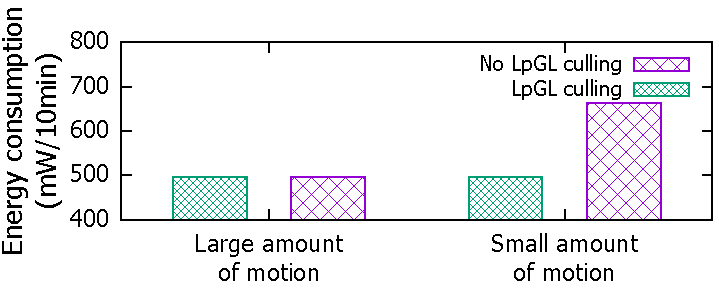
\includegraphics[width=0.8\linewidth]{cullingEnergy}
    \vspace{-2ex}
    \caption{Impact of culling on the HoloLens energy consumption for different head motion samples.}
    \label{fig:culling-energy}
\end{figure}


%%%%%%%%%%%%%%%%%%%%%%%%%%%%%%%%% 80 CHAR %%%%%%%%%%%%%%%%%%%%%%%%%%%%%%%%%%%%%%

\spar{{\myit} Culling}:
%
To verify the impact of {\myit}'s culling on energy, we test with 
and without {\myit}'s culling component turned on. When it is off, only the 
graphics stack's default culling is used. 
%
\fig\ref{fig:culling-energy} shows that, with small amounts of head motion,
{\myit}'s culling feature indeed offers significant ($\sim$27\%) energy savings.
%
In this case, all 20 blocks will be drawn on the scene for most of the time, 
but a subset of the blocks will move out of the FOV
for short periods when the user is moving the blocks.
This is the time when {\myit}'s culling successfully suppresses their 
processing and lowers the energy consumption. 
%
Unexpectedly, however, when there is large amount of head motion, the default 
culling also shows low energy usage rate.
%
This an effect caused by the peculiarity of our application scenario.
Once a user makes large head movements, already stacked 
existing blocks move out of the scene for long periods.
%(similar to the effect in \figs\ref{fig:framedynamics-trace-large} 
%and~\ref{fig:framedynamics-trace-small}). 
%
At this point, due to the simplicity of the scene \rev{(with no backgrounds)}, 
the graphics pipeline is not doing much work even without {\myit}. Therefore, 
both options consume the baseline energy despite {\myit} suppressing tasks up
to the vertex shader.
%
But as the small amount of head motion case shows, {\myit}'s enhanced culling
is beneficial when there are sufficient number of objects in the scene and the
system operates at the boundary of the baseline workload limit.

%%%%%%%%%%%%%%%%%%%%%%%%%%%%%%%%% 80 CHAR %%%%%%%%%%%%%%%%%%%%%%%%%%%%%%%%%%%%%%

\begin{figure}[t]
    \centering
    \vspace{-1ex}
    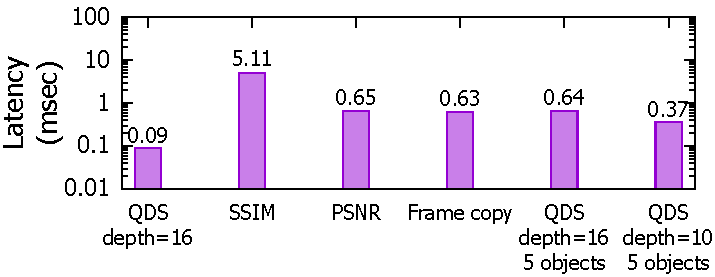
\includegraphics[width=0.8\linewidth]{dynamicScoringLatency}
    \vspace{-2ex}
    \caption{Latency comparisons for different scene dynamics scoring methods
            (Quad-tree based dynamics scoring (QDS), SSIM, and PSNR).}
    \label{fig:dynamicScoringLatency}
\end{figure}

%%%%%%%%%%%%%%%%%%%%%%%%%%%%%%%%% 80 CHAR %%%%%%%%%%%%%%%%%%%%%%%%%%%%%%%%%%%%%%

\subsection{Computational Latency}


An important factor we should consider besides energy is the latency of the 
algorithms we've designed in {\myit}. If algorithms take long to execute, 
this too can affect the user experience and disrupt application requirements.
%
\fig\ref{fig:dynamicScoringLatency} plots the latencies for computing the 
screen dynamics using various methods. Our scheme, QDS, is compared with 
widely used image-based frame dynamics computing methods such as SSIM and PSNR.
%
To compute at the same granularity, we set $d_Q$ as 16. Here we use a scene 
which consists of a cube in the center. Comparing the first three bars show 
that the latency of QDS-based frame dynamics computation ($\sim90~\mu$sec per frame)
is significantly lower than the SSIM ($\sim$55x) and PSNR ($\sim$7x).
%
The fourth bar, in which we plot the time spent by the PSNR and SSIM schemes 
while copying the frame buffer contents from the GPU to the memory for dynamics 
computation, shows that a large portion of this latency (the majority for 
PSNR; 0.63 of 0.65 msec) is wasted on the memory copy process.
%
This result suggests that our geometry-based approach can
outperform the image-based algorithms. It is especially true for
AR HMDs given that only a small portion of the scene is usually drawn
on the screen compared to VR or mobile AR applications. 


Next, we try adding four additional cubes to the scene and compute the latency
for QDS. The fifth bar in \fig\ref{fig:dynamicScoringLatency} shows that when
more quad trees are constructed to support more objects, the latency of QDS 
increases rapidly.
Nevertheless, from the sixth bar we can see that lowering $d_Q$ to 10 (from 16)
shows a much decreased latency of 0.37 msec.

\begin{figure}[t]
    \centering
    \vspace{-1ex}
    \subfigure[Binary tree construction latency for varying tree depths]{
        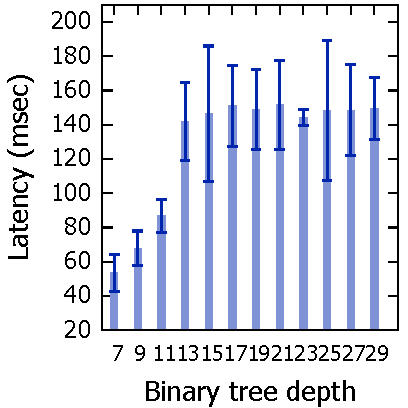
\includegraphics[width=0.41\linewidth]{octreeLatency}
        \label{fig:octree-latency}
    }
    \hfill
    \subfigure[Simplified Stanford Bunnies using binary tree-based mesh simplification]{
        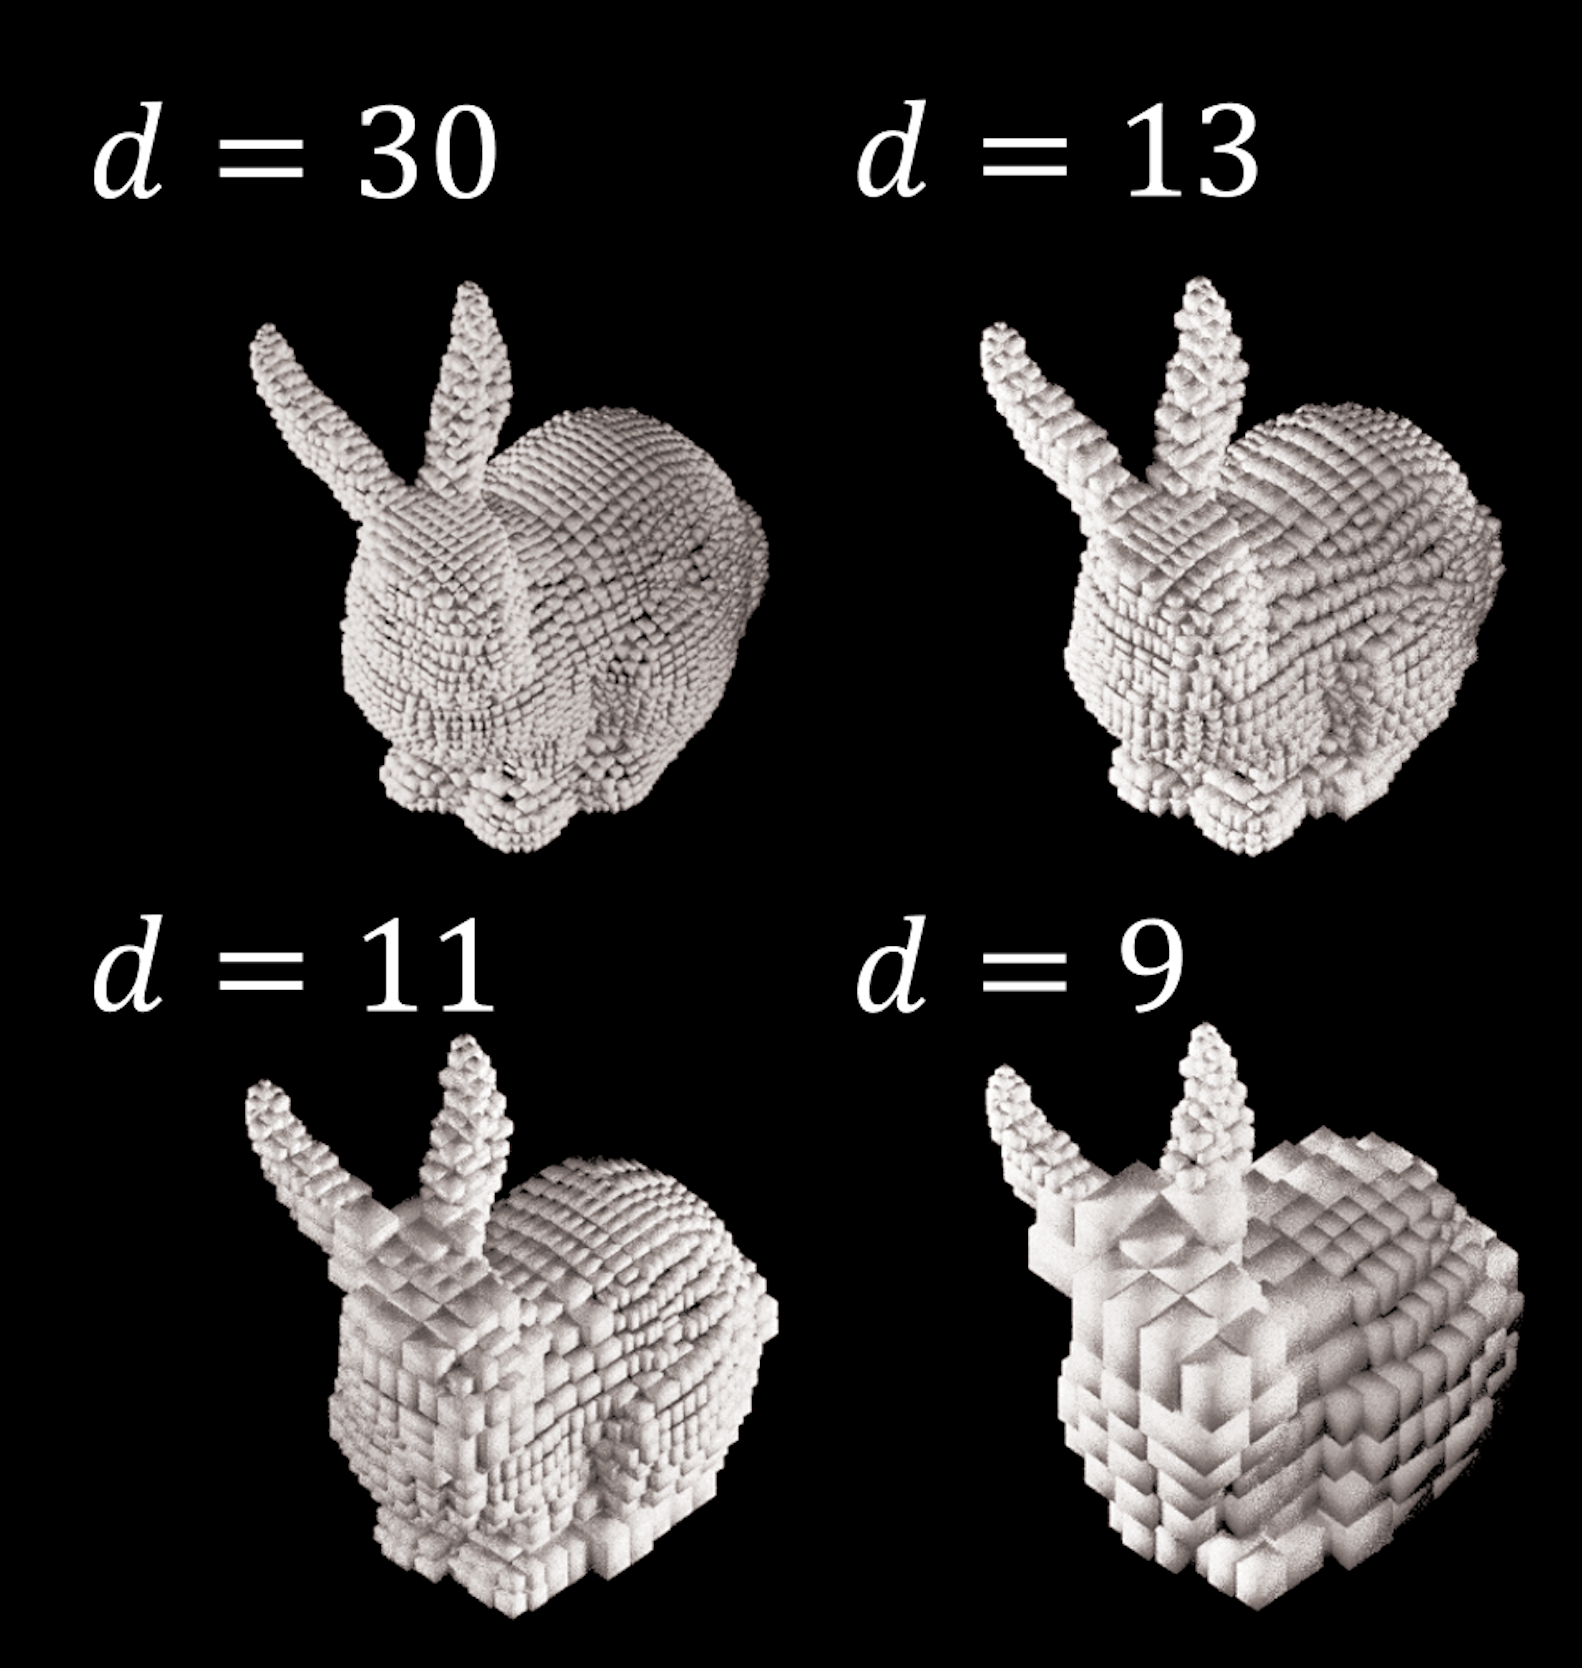
\includegraphics[width=0.39\linewidth]{simplifiedBunnies}
        \label{fig:octree-bunny}
    }
    \vspace{-2ex}
    \caption{Binary tree construction latency for Stanford Bunny and 
        the results of mesh simplification.}
    \label{fig:octreeConstructionLatency}
\end{figure}

%\begin{figure}[t]
%    \centering
%    %\includegraphics[width=1\linewidth]{}
%    \caption{The simplified bunny 3D models}
%    \label{fig:simplifiedBunnies}
%\end{figure}

The latency introduced by the binary tree construction process is presented in 
\fig\ref{fig:octree-latency} for the full-resolution Stanford Bunny with 
$\sim$69K triangles while varying $d_B$.
%
We also present the outcome of the binary tree-based mesh simplification in 
\fig\ref{fig:octree-bunny} for different depths. Results show that the mesh 
simplification process for a full-resolution Stanford Bunny takes less than 
$\sim$80~msec for $d_B\le$11 and the latency converges (at $\sim$140~msec) for 
higher $d_B$ values.
%
Given that these simplified objects will be displayed for objects that are 
\textit{out of} the user's focus range (by more than $\epsilon^\circ$) we can 
see that voxelization effectively simplifies the target objects.
%
%Note that  given the binary tree depth of $d_B$ and $n$ triangles,
%the theoretical complexity is $O((2n)^{d_B})$. Nevertheless, at each step
%{\myit} only checks for vertex inclusions in the binary tree; thus, the
%quantitative results are small enough to induce minimal effect on the user
%experienced latency. 


%%%%%%%%%%%%%%%%%%%%%%%%%%%!!DO NOT USE!!!!%%%%%%%%%%%%%%%%%%%%%%%%%%%%%%%%%%%%%
%%%%%%%%%%%%%%%%%%%%%%%%%%%!!DO NOT USE!!!!%%%%%%%%%%%%%%%%%%%%%%%%%%%%%%%%%%%%%
% 먼저 우리는 환아를 대상으로 실험을 진행하기 전, 20대 30대 성인 남녀 x 명을 대상으로 사전 실험을 진행했다.
% 이번 실험에서는 설문을 더 잘 이해할 수 있는 성인들을 대상으로 Block stacking 실험을 진행하여 Strabismus Patients 환아 들에게 적용할 실험의 feasibility를 알아보았고 {\myit} 적용으로 인해 발생하는 퀄리티 저하에 대해 미리 알아보기 위하여 간단한 survey를 진행했다.
% 실험의 protocol은 다음과 같았다. 먼저 block stacking 게임을 실행 시킨 뒤, 조작법을 가르쳐 주어 AR 환경에서의 조작에 익숙해 질 수 있도록 했다. 그 후 세 번의 실험 인스턴스를 수행했다. 하나는 {\myit}를 적용하지 않은 게임, {\myit}를 적용하되 quad-tree dynamics scoring에 대해 높은 감도에서 반응하는 게임, 마지막으로 {\myit}를 적용하되 quad-tree dynamics scoring에 대해 낮은 감도에서 반응하는 게임이었다. 만약 감도가 낮다면 dynamic score가 굉장히 높아야지만 반응하게 되므로 에너지 소모는 아낄 수 있지만 사용자 경험을 희생하게 된다. 반대로 감도가 높다면 조금만 움직이더라도 framerate이 높아져 사용자 경험에는 좋지만 에너지 소모를 줄일 수 있는 가능성은 낮아진다.
% 각 instance를 마친 뒤 우리는 사용자 경험에 대한 설문을 진행했다. 설문의 내용은 다음과 같았다. 1) 눈이 아프지는 않았는가? 2) 불편한 정도를 점수로 나타내면? 3) 어지러움을 느꼈나? 4) 보이는 그림이 뚜렷했나? 5) 화면이 부드러웠나?
% 결과는 다음과 같았다. 먼저, 대부분의 피실험자들이 눈의 고통이나 어지러움을 느끼지 못했다. 불편함에 대해서는 화면의 quality 저하가 영향을 주기보다는 constant하게 AR HMD 환경 자체에 불편함을 느끼는 사람들이 x%였다. 또한 일부 집단은 framerate의 변화에 따른 화면의 부드러움 변화를 인지했지만, 의미있는 다수가 이러한 변화를 인지하지 못했다.
% 이러한 실험을 통해서 우리는 {\myit}가 사용자 경험에 critical한 영향을 주는 것은 아니라고 결론을 내릴 수 있다. //먼저, 대부분의 피실험자이 감도에 상관없이 비슷한 대답을 했다는 것을 알 수 있었다. 수치적으로 보면 (1), (2)번 질문에서는 거의 유사한 대답얻을 수 있었고, (3)번 질문에 대해서는 아주 조금 높지만 마찬가지로 거의 유사한 1.5~2정도 사이의 대답을 얻을수 있었다. 심지어 어떤 case에서는 낮은 감도에서 오히러 더 물체가 또렸하게 보였다는 대답을얻었다.어 을 수 있 심지어 낮은 감도에서 보이는 그림이 더 뚜렷했다고 대답을 한 경우도 있었다. 따라서 우리는 이정도 감도의 변화는피 실험자들의 사용성에 영향을 주지 않는다는 결론을 내릴 수 있었다.
%%%%%%%%%%%%%%%%%%%%%%%%%%%%%%%%%%%%%%%%%%%%%%%%%%%%%%%%%%%%%%%%%%%%%%%%%%%%%%%%
%%%%%%%%%%%%%%%%%%%%%%%%%%%%%%%%%%%%%%%%%%%%%%%%%%%%%%%%%%%%%%%%%%%%%%%%%%%%%%%%

\subsection{3D Block Stacking Application}
\label{sec:app}

%%%%%%%%%%%%%%%%%%%%%%%%%%%%%%%%% 80 CHAR %%%%%%%%%%%%%%%%%%%%%%%%%%%%%%%%%%%%%%

\raj{merge this into the evaluation section for the user study}

To evaluate the usability of {\myit} on a real application at the user level,
we designed an AR application for implicitly measuring the stereoscopsis level 
of children with strabismus using AR HMDs, and performed an Institutional Review
Board (IRB)-approved pilot study with strabismus (i.e., crossed eye) patients in
the ophthalmology department at a university hospital.
%
The purpose of our pilot study was to validate changes in user-perceived
object rendering quality when applying {\myit} with different configurations.


Traditionally, devices such as keratometers are used to measure the 
stereoscopsis level. However, these devices are bulky and cannot effectively 
gain the attention of children to focus during the measurements.
%
For this reason, the clinical staff asked for a more interactive and engaging 
game to measure children's stereoscopsis levels, and we designed an AR-based 
game where the children were asked to stack 3D blocks using Microsoft HoloLens%
\footnote{We used DirectX as the underlying native graphics library}
(c.f., \fig\ref{fig:hololens}).


The block stacking game operates as follows.
%
When the application starts, a white cube palette is displayed.
Once the user visually focuses on the cube, the user is asked to press a clicker
device and move the object in the 3D space.
%
Using such movements, the user is asked to stack all cube blocks on the display.
The performance of moving the objects becomes an indirect measure of the 
stereoscopsis level. 
%
We designed this game and user study to confirm if {\myit} makes proper 
transitions in frame rate or changes in object quality, while minimally 
affecting the user perceived quality.
%
Furthermore, we also gathered statistics on the amount of energy 
that can be saved by applying {\myit} to real-world applications%
\footnote{A sample video of the application and its interaction with {\myit} is
available, and we will provide the URL after the anonymous review process.
%at \todo{http://}
}.

%\jk{Let's make a recording of the task and share on Youtube.}



%%%%%%%%%%%%%%%%%%%%%%%%%%%%%%%%%%%%%%%%%%%%%%%%%%%%%%%%%%%%%%%%%%%%%%%%%%%%%%%%%


% 이러한 실제 stereoscopsis의 측정에 앞서, 우리는 AR HMD의 사용성에 대해서 면밀히 검토할 필요가 있었다. 특히 우리의 실험 대상은 어린이 환자들이었고, 이러한 환자들이 새로운 환경인 HMD 환경을 쉽게 이용할 수 있는지는 큰 챌린지 중 하나였다. 구체적으로 살펴보면 첫번째로 조작의 편의성을 확인해야 했다. Microsoft HoloLens로 조작할 수 있는 주요 방법은 손가락을 통한 gesture 인식과 external 장비인 clicker 가 있다. gesture 인식의 경우 HoloLens에 부착되어 있는 depth sensor에 손이 보여야 하는 문제가 있고 클릭의 정밀도가 낮다는 단점이 있는 반면, clicker를 이용하면 click 이라는 액션이 명확하다는 장점이 있기 때문에 우리는 clicker를 사용하기로 했다. 두번째로 HMD라는 경험이 환자들에게 어떻게 느껴지는지 인 지점이 있었다. 알려져 있기로 HMD 경험이 눈의 고통을 주기도 하고, 어지러움을 야기할 수도 있고, 불편함을 주기도 했는데 실제로 어린이 환자에게 AR 응용을 적용됐을 때 어떤 경험을 주는지 확인해 보는 것은 추후 AR 응용을 개발하는데에 좋은 information이 될 수 있다.  마지막으로 어린이 환자를 위한 측정 방법과 설문의 난이도를 고려하는 것이 중요했다. block stacking이라는 간단한 동작이지만 이러한 동작이 어린이들, 특히 환아들에게 어려울 수 있고 이러한 과정에 대한 설문을 하는 과정도 쉬운 언어를 통해서 진행이 되어야 했다.

%%%%%%%%%%%%%%%%%%%%%%%%%%%%%%%%% 80 CHAR %%%%%%%%%%%%%%%%%%%%%%%%%%%%%%%%%%%%%%

%\subsection{Application-level View Frustum Culling}

% 이번 섹션에서는 draw call을 줄이기 위한 방법인 user level view frustum culling의 방법에 대해 구체적으로 설명한다. 이전 섹션에 말했 듯, culling은 visibility를 판단하는 작업이다. 그래픽스 파이프라인에서는 view frustum culling이라고 불리는 작업을 수행하는데, 이는 카메라 정보, 그 중에서도 종횡비 시야각, 그리고 최소 가시거리, 최대 가시거리 정보를 통해 frustum을 만들고, 렌더링하는 물체들이 frustum의 바깥으로 나가는지 그렇지 않은지를 판단하는 방법들이다. 이러한 방법을 통해 화면에 보이지 않는 triangles를 판단하고, 이후 pipeline 작업에서는 해당 triangles를 배제해서 성능 향상을 이룬다.

% 하지만 그럼에도 불구하고 system level이 아닌 application level에서의 view frustum culling은 필요하다. 그 이유는 렌더링 되지 않는 draw call도 에너지 소모에 영향을 주기 때문이다. 그 이유는 view frustum culling이 일어나는 시점의 문제에 있다. draw call이 불리면 graphics pipeline은 모든 그려야 하는 vertices를 vertex shader를 통해서 병렬적으로 transformation한다. 이 이후 시점에서 view frustum culling이 일어난다. 즉, 실제로 그려지게 될지 모르는 상태에서 연산을 해야 한다는 것이다. 이로 인해 높은 the number of triangles를 가진 모델의 경우 자원을 크게 낭비하게 된다.

% 우리는 다음과 같은 방법을 통해 user level에서 light-weight view frustum culling을 진행한다. gpu에서의 view frustum culling은 mesh의 모든 triangles에 대해서 진행되기 때문에 비용이 비싸다. 하지만 우리는 우리는 mesh의 triangles가 아닌 initialization 시에 만든 mesh의 bounding box를 이용한다. 이러한 bounding box는 모델의 전체를 bound하고 있기 때문에 만약 camera가 바라보고 있는 방향기준으로 시야각 바깥에 bounding box가 있다면 이 모델이 보일 가능성이 없다고 생각할 수 있다. 이러한 케이스에 대해서는 해당 모델에 대한 draw call을 호출하지 않음으로 인해서 에너지 소모를 줄일 수 있다.


%%%%%%%%%%%%%%%%%%%%%%%%%%%%%%%%% 80 CHAR %%%%%%%%%%%%%%%%%%%%%%%%%%%%%%%%%%%%%%

\begin{comment}

To explain the implementation details of the bounding box projection process, we take as example, once again, the Stanford Bunny. Say that there is a Stanford Bunny and we want to compute the three metrics (i.e., XXX, XXX, and XXX) discussed above. Given the vertices and topology information for the bunny rendering, we receive the transformation matrix from the application to apply the target transformation (e.g., scaling, rotation, translation) to the vertices. On the application's perspective, as a result of the transformation process, a vertex $V$ will be located at $(x,y,z)$ from the origin point $(0,0,0)$. Here we say that $V$ is transformed in to world-space. \jk{huh???}

% 간단한 예로 화면에 stanford bunny가 그려져 있고, 우리가 위에서 정의한 세가지 방법들을 계산하기 위해 유저 입장에서 이 bunny가 어떻게 보이는지를 계산하고 싶다. 렌더링을 하기 위한 vertices와 topology information이 있을 때, 이에 원하는 transformation (e.g. scaling, rotation, translation)을 적용하기 위해 transformation matrix를 application 단으로부터 받아서 vertices에 곱해준다. 이렇게 transform된 vertices는 중 하나의 vertices v 는 application 입장에서 origin, 즉 (0, 0, 0)을 기준으로 (x, y, z)에 위치하게 된다. 이때의 v를 v is transformed into world space. 라고 표현한다. 이 상태에서는 user 의 

\end{comment}





\subsection{Pilot Study with Strabismus Patients}
\label{sec:pilot-study}

Finally, using the application discussed in Section~\ref{sec:app}, we performed 
an IRB-approved pilot study with a total of eight children participants 
(ages 7-10), of which four were diagnosed with strabismus and the other four 
visited the hospital for post-surgical check ups.
%
The purpose of this study was to validate changes in user-perceived object
rendering quality (including user experience) when applying {\myit} with different target quality levels.
%
%\rev{and also to verify that applying {\myit} did not disturb the user experience within the application.}


We started our study by teaching the children how to play the block stacking 
game, and had them get used to controlling objects in the AR environment.
%
In the actual experiment phase, we had each child play three versions of the
block stacking application: one version without {\myit}, {\myit} with 
low-sensitivity QDS thresholds, and {\myit} with high-sensitivity QDS thresholds.
%
This information was not disclosed to the participants and the testing order was
randomized to remove any bias.


% Note that the contents of this game is very simple;
% therefore, there is only a minimal amount of energy savings from the frame rate
% control and mesh simplification. Rather than analyzing the energy usage,
% the purpose was to verify that applying {\myit} did not disturb the user 
% experience within the application context.
%
Using a visual analogue scale (VAS) type of survey (1-5 scale), we collected 
information on (1) whether the participant felt any dizziness, (2) the clarity 
of the blocks, and (3) how comfortable the game was to the eyes.
%
We note that all participants responded with answers of similar patterns
regardless of the test scenario.
%
Quantitatively, for questions (1) and (3), most participants answered with 
a score of 1, indicating that the system was comfortable and there were no 
dizziness. Answers for question (2) were in the range of 1.5-2, suggesting that
the clarity was not perfect but acceptable. Surprisingly, some participants 
answered that {\myit} with low-sensitivity showed the most clear images.
Given that we randomized the experiment sequence, this suggests that frame 
rate changes (for our application) gave minimal effect to the
usability and object quality.


\rev{
We acknowledge that eight children participants are not a large enough and
representative user population to generalize our user study given the broad 
range of AR applications.
%
However, they are unbiased, and we emphasize that the study was performed 
for a real use case at the hospital.
%
We plan to extend our case study to a more diverse set of applications with
larger subjects as part of our future work.
}


%%%%%%%%%%%%%%%%%%%%%%%%%%%%%%%%% 80 CHAR %%%%%%%%%%%%%%%%%%%%%%%%%%%%%%%%%%%%%%


